% VLEN sweep line chart: x=VLEN, y=instret (total KEM)
% Multiple lines for HQC-128/192/256 (vector_zvk variant)
% Source: results/simulation/benchmarks/vlen_scaling/*-vector-zvk_latest.csv (commit 7c8d219)
\tikzsetnextfilename{ch8-results-vlen-sweep-line}
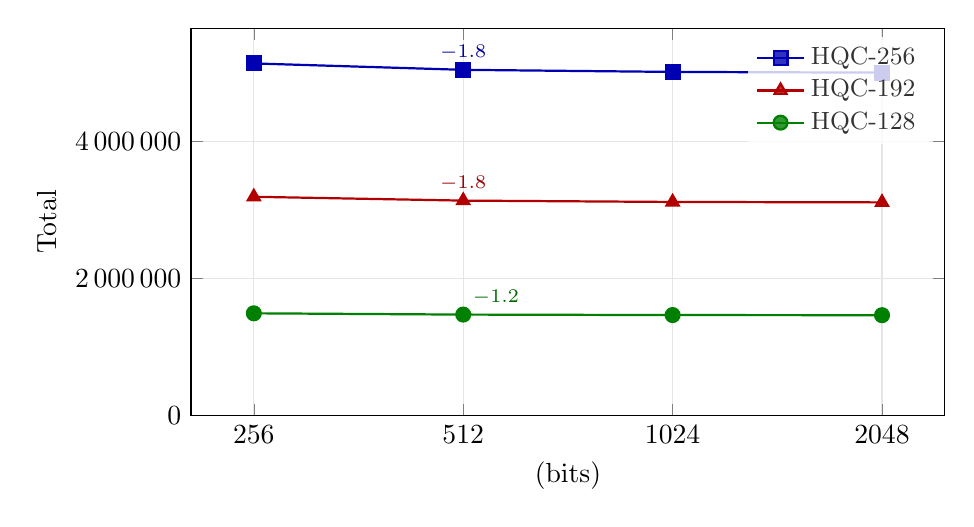
\begin{tikzpicture}
\begin{axis}[
  width=0.92\linewidth,
  height=6.5cm,
  xlabel={\VLEN (bits)},
  ylabel={Total \KEM \instret},
  xmode=log,
  log basis x=2,
  xtick={256, 512, 1024, 2048},
  xticklabels={256, 512, 1024, 2048},
  ymin=0,
  scaled y ticks=false,
  y tick label style={/pgf/number format/fixed,
                      /pgf/number format/1000 sep={\,}},
  legend style={at={(0.98,0.98)}, anchor=north east,
                font=\small, draw=none, fill=white, fill opacity=0.8},
  grid=major,
  grid style={gray!20},
  every axis plot/.append style={thick, mark size=2.5pt},
  cycle list name=color list,
]

% HQC-256
\addplot[blue!70!black, mark=square*] coordinates {
  (256, 5138700)
  (512, 5045386)
  (1024, 5014831)
  (2048, 5004353)
};
\addlegendentry{HQC-256}

% HQC-192
\addplot[red!70!black, mark=triangle*] coordinates {
  (256, 3192507)
  (512, 3136588)
  (1024, 3116877)
  (2048, 3110691)
};
\addlegendentry{HQC-192}

% HQC-128
\addplot[green!50!black, mark=*] coordinates {
  (256, 1491550)
  (512, 1473002)
  (1024, 1466123)
  (2048, 1464102)
};
\addlegendentry{HQC-128}

% Annotation: main gain at VLEN=512
\node[anchor=south, font=\scriptsize\itshape, text=blue!60!black]
  at (axis cs:512, 5045386) {$-\pct{1.8}$};
\node[anchor=south, font=\scriptsize\itshape, text=red!60!black]
  at (axis cs:512, 3136588) {$-\pct{1.8}$};
\node[anchor=south west, font=\scriptsize\itshape, text=green!40!black]
  at (axis cs:512, 1473002) {$-\pct{1.2}$};

\end{axis}
\end{tikzpicture}
